\section{Relational Colour Refinement for structures with functions}
\label{sec:RelationalColourRefinemetForStructuresWithFunctions}

\subsection{Naive Encoding of functions}
\label{Sec::NaiveEncodingOfFunctions}

A simple way to apply relational colour refinement to non-relational structures is, to encode the functions as relations.
Formally we transform a signature $\sigma$ that includes function symbols to a new signature $\sigma'$: 
For every relation symbol $R\in \sigma$, we introduce a relation symbol $R\in \sigma'$ with the same arity and for every function symbol $f\in\sigma$ with arity $k$, we introduce a relational symbol $R_f\in\sigma'$ of arity $k+1$.

Semantically, a structure $\mathfrak A$ of signature $\sigma$ can then be encoded as a structure $\mathfrak A'$ of signature $\sigma'$ and with the same universe as $\mathfrak A$. 
For every relational symbol $R\in\sigma$ we set $R^{\mathfrak A'}\coloneqq R^{\mathfrak A}$ and for every function symbol $f\in\sigma$ of arity $k$ there exists a relation symbol $R_f\in\sigma'$ and we set $R_f^{\mathfrak A}\coloneqq \{\mathbf xy : f^{\mathfrak A}(\mathbf x)=y\}$ where $\mathbf x$ is a tuple of arity $k$.

This procedure encodes a non-relational structure as a relational one, on which Relational Colour Refinement can now be performed.
As such we say, that the Naive Relational Colour Refinement (nRCR) distinguishes two structures $\mathfrak A$ and $\mathfrak B$ if, and only if, RCR distinguishes their naive encodings $\mathfrak A'$ and $\mathfrak B'$.
However, this results in a very weak logical characterisation, that does not allow nesting of terms, namely the nesting-free-fragment of $\GFC$.

\begin{definition}[$\mathsf{nfGF}(\mathsf C)$]
	Consider the definition of $\GFC$ given in \ref{}.
	We obtain the nesting-free fragment, by allowing $f(\mathbf x)=y$ as a further atomic formula.
	Concretely, the only allowed atomic formulae are of the form $R(x_1,\dots,x_\ell)$, $x=y$ and $f(x_1,\dots,x_\ell)=y$, where $f$ has arity $\ell$, $\free{f(x_1,\dots,x_\ell)=y}=\{x_1,\dots,x_\ell\}$ and $\gd{f(\mathbf x)=y}=0$.
	
	The remaining definitions stay the same.
\end{definition}

\begin{theorem}
	\label{thm:ThmA}
	The two following statements are equivalent:
	\begin{enumerate}
		\item nRCR distinguishes $\mathfrak A$ and $\mathfrak B$.
		\item There exists a sentence $\phi\in \mathsf{nfGF}(\mathsf C)$ such that $\mathfrak A\models \phi$ and $\mathfrak B\not\models \phi$.
	\end{enumerate}
\end{theorem}
\begin{proof}
	1. $\Rightarrow$ 2.:
	By definition, $\mathfrak A$ and $\mathfrak B$ are distinguished by nRCR if, and only if, $\mathfrak A'$ and $\mathfrak B'$ are distinguished by RCR.
	Using the result of \cite{scheidt2025ColorRefinement}, we obtain a sentence $\varphi'\in\GFC$ that distinguishes the encoded structures.
	Via a structural induction on the formula, we can now translate $\varphi'$ into a formula $\phi\in \mathsf{nfGF}(\mathsf C)$
	This can be achieved by replacing formulae $R_f(x_1,\dots,x_\ell,y)$ by $f(x_1,\dots,x_\ell)=y$ for function symbols $f\in\sigma$ and letting everything else stay the same.
	
	2. $\Rightarrow$ 1.:
	When considering $\mathsf{nfGF}(\mathsf C)$, one can find that the transformation done at the end of the first direction can be applied in reverse.
	This then leads to a distinguishing sentence in $\GFC$ and with \cite{scheidt2025ColorRefinement} to a distinguishing colouring of the encoded structures, which by definition is a distinguishing colouring for the structures themselves.
\end{proof}

While the above theorem results in a nice characterisation of the naive encoding, the nesting of terms is often very desired when using functions.
However, it can be shown that nesting is too powerful for the naive encoding.

Consider the two structures $\mathfrak A$ and $\mathfrak B$ of signature $\sigma=\{f/1\}$ which can be seen in \cref{NaiveEncodingCounterexample}.
Formally they are defined as $\mathfrak A=(A,f^{\mathfrak A})$ and $\mathfrak B = (B, f^{\mathfrak B})$ where

\begin{alignat*}{4}
	A=&\{a_1,a_2,a_3,a_4,a_5,a_6\}, &&  && B=&&\{b_1,b_2,b_3,b_4,b_5,b_6\},\\
	f^{\mathfrak A}=&\{a_1\mapsto a_2, a_2\mapsto a_3, a_3 \mapsto a_1, && \qquad \text{and} \qquad && f^{\mathfrak B}=&&\{b_1 \mapsto b_2, b_2 \mapsto b_3, b_3 \mapsto b_4, \\
	&\phantom{\{} a_4\mapsto a_5, a_5\mapsto a_6, a_6\mapsto a_4 \} &&  && && \phantom{\{} b_4 \mapsto b_5, b_5 \mapsto b_6, b_6 \mapsto b_1\}
\end{alignat*}

\begin{figure}
	\centering
	\begin{multicols}{2}
		\begin{tikzpicture}
			\node[state] (a1) {$a_1$};
			\node[left=of a1, xshift=-0.5cm] (label) {$\mathfrak A$:};
			\node[state, below left=of a1] (a3) {$a_3$};
			\node[state, below right=of a1] (a2) {$a_2$};
			\node[state, below =of a3] (a4) {$a_4$};
			\node[state, below =of a2] (a5) {$a_5$};
			\node[state, below left=of a5] (a6) {$a_6$};
			\draw 
			(a1) edge[->, above] node{$f^{\mathfrak A}$} (a2)
			(a2) edge[->, below] node{$f^{\mathfrak A}$} (a3)
			(a3) edge[->, above] node{$f^{\mathfrak A}$} (a1)
			(a4) edge[->, above] node{$f^{\mathfrak A}$} (a5)
			(a5) edge[->, below] node{$f^{\mathfrak A}$} (a6)
			(a6) edge[->, below] node{$f^{\mathfrak A}$} (a4);
		\end{tikzpicture}
		\begin{tikzpicture}
			\node[state] (b1) {$b_1$};
			\node[left=of b1, xshift=-0.5cm] (label) {$\mathfrak B$:};
			\node[state, below left=of b1] (b6) {$b_6$};
			\node[state, below right=of b1] (b2) {$b_2$};
			\node[state, below =of b2] (b3) {$b_3$};
			\node[state, below =of b6] (b5) {$b_5$};
			\node[state, below left=of b3] (b4) {$b_4$};
			\draw 
			(b1) edge[->, above] node{$f^{\mathfrak B}$} (b2)
			(b2) edge[->, right] node{$f^{\mathfrak B}$} (b3)
			(b3) edge[->, below] node{$f^{\mathfrak B}$} (b4)
			(b4) edge[->, below] node{$f^{\mathfrak B}$} (b5)
			(b5) edge[->, left] node{$f^{\mathfrak B}$} (b6)
			(b6) edge[->, above] node{$f^{\mathfrak B}$} (b1);
		\end{tikzpicture}
	\end{multicols}
	
	\caption{Two $\sigma$-structures $\mathfrak A$ and $\mathfrak B$ which can be distinguished by $\GFC$, but not by $\operatorname{nRCR}$.}
	\label{NaiveEncodingCounterexample}
\end{figure}

Consider the formula $\phi=\exists^{\geq 1} x.(f(f(f(x)))=x)$ which utilizes term nesting to find a cycle of length three.
It is obvious that $\mathfrak A \models \phi$ and $\mathfrak B\not\models \phi$.
However, when encoding the two structures with the naive method described above, one finds that nRCR cannot distinguish them.
Therefore, term nesting is too powerful for the naive encoding.

A method that allows for the nesting of terms will be described in the following section.


\subsection{Using the transitive expansion} 

As a first remark we note that we only consider unary functions in this section.
The key idea will be, to encode a function $f$ as a family of relations, which then can capture the notion of nesting function applications.
However, a bound on the alternation of different function symbols is necessary to ensure that the expanded signature is still finite, thus we will fixate a maximal alternation depth when discussing our new variant of $\RCR$.
Let us now concretely define, how we expand the signature.

\begin{definition}[Transitive Expansion]
	Let $\sigma\coloneqq \sigma_{\operatorname{Rel}} \operatorname{\dot{\cup}} \sigma_{\operatorname{Func}}$ be a signature with relation symbols $\sigma_{\operatorname{Rel}}$ and unary function symbols $\sigma_{\operatorname{Func}}$ and let $\mathfrak A$ be a structure of signature $\sigma$ with $\Vert \mathfrak A \Vert=n$.
	For readability, we define the family of sets of alternations of function applications $\operatorname{Alters}_n^0(\sigma)\coloneqq\{\operatorname{id}\}$ and
	\begin{align*}
		\operatorname{Alters}^k_{n}(\sigma)\coloneqq \operatorname{Alters}^{k-1}_{n}(\sigma)\cup\{f_1^{m_1}f_2^{m_2}\dots f_k^{m_k} : & f_1f_2\dots f_k\in (\sigma_{\operatorname{Func}})^k \\ 
		& \land 0 < m_i \leq n \text{ for } i \in [k] \\ 
		& \land \forall i\in\{1,\dots,k-1\} . f_{i-1}\neq f_i \neq f_{i+1}\}.
	\end{align*}
	We will now fixate an arbitrary $k\in\mathbb N$ which will be our bound on the alternation depth and will define a new signature $\widetilde{\sigma}$ as well as a structure $\widetilde{\mathfrak A}$ of said signature, which will be the transitive expansion with alternation depth $k$ of $\mathfrak{A}$.
	For $k\in\mathbb N$, $\alpha,\beta,\alpha_1,\dots,\alpha_\ell\in \operatorname{Alters}^k_n(\sigma)$ and a $R\in \sigma_{\operatorname{Rel}}$ with arity $\ell$, we define the binary relation
	$$\operatorname{Eq}_{\alpha,\beta}^{\widetilde{\mathfrak A}}\coloneqq \{(a,b) : \alpha^{\mathfrak A}(a)=\beta^{\mathfrak A}(b)\},$$
	and the relation of arity $\ell$
	$$R_{\alpha_1,\dots,\alpha_\ell}^{\widetilde{\mathfrak A}} \coloneqq \{(a_1,\dots,a_\ell) : (\alpha_1^{\mathfrak A}(a_1),\dots,\alpha_\ell^{\mathfrak A}(a_\ell))\in R^{\mathfrak A}\}.$$
	We now define the transitive expansion with alternation depth $k$ signature $\widetilde{\sigma}$, where 
	\begin{align*}
		\widetilde{\sigma}\coloneqq & \{\operatorname{Eq}_{\alpha,\beta}: \alpha,\beta\in\operatorname{Alters}^k_n(\sigma)\}, \\
		& \operatorname{\dot{\cup}} \{R_{\alpha_1,\dots,\alpha_\ell} : R\in \sigma_{\operatorname{Rel}},\operatorname{ar}(R)=\ell \text{ and } \alpha\in \operatorname{Alters}^k_n(\sigma)\}.
	\end{align*}
\end{definition}

Since the following definitions will depend on this construction, let us consider an example.
We define the signature $\sigma=\{R,f,g\}$ where $R$ is a unary relation symbol and $f$ and $g$ are unary function symbols.
Now consider a $\sigma$ structure $\mathfrak A=(A,\sigma)$ with $A=\{a,b\}$, $R^{\mathfrak A}=\{a\}$, $f^{\mathfrak A}=\{a\mapsto b, b\mapsto a\}$ and $g^{\mathfrak A}=\{a\mapsto a, b\mapsto b\}$.
A graphical representation of $\mathfrak A$ can be found in \cref{TransitiveExpansionExample}.
For the sake of simplicity we will define the transitive expansion with alternation depth $1$ and because $\Vert\mathfrak A\Vert=2$ we will use $\operatorname{Alters}^1_2(\sigma)$ to do so.
We see that $\operatorname{Alters}^1_2(\sigma)=\{\operatorname{id}, f,f^2,g,g^2\}$ and as such 
$$\widetilde{\sigma}=\{R_{\operatorname{id}}, R_{f}, R_{f^2}, R_g, R_{g^2}, \operatorname{Eq}_{\operatorname{id},\operatorname{id}}, \operatorname{Eq}_{\operatorname{id},f}, \operatorname{Eq}_{\operatorname{id}, f^2}, \dots, \operatorname{Eq}_{g^2, g^2}\}.$$
Because of the relatively large size of $\widetilde{\sigma}$, we will only give the formal definitions for a few relations, while the rest of the relations in $\widetilde{\mathfrak A}$ can be seen in \cref{TransitiveExpansionExample}.
We find that $R^{\widetilde{\mathfrak A}}_{\operatorname{id}}=R^{\widetilde{\mathfrak A}}_{f^2}=R^{\widetilde{\mathfrak A}}_g=R^{\widetilde{\mathfrak A}}_{g^2}=\{a\}$ and that $R^{\widetilde{\mathfrak A}}_f=\{b\}$.
Additionally, $\operatorname{Eq}^{\widetilde{\mathfrak A}}_{g,\operatorname{id}}=\operatorname{Eq}^{\widetilde{\mathfrak A}}_{g^2,\operatorname{id}}=\{(a,a),(b,b)\}=\operatorname{Eq}^{\widetilde{\mathfrak A}}_{\alpha,\alpha}$ for all $\alpha\in\operatorname{Alters}^1_2(\sigma)$.
To give another example, we have $\operatorname{Eq}^{\widetilde{\mathfrak A}}_{g,f}=\operatorname{Eq}^{\widetilde{\mathfrak A}}_{g^2,f}=\{(a,b),(b,a)\}$.
The definitions of all $\operatorname{Eq}^{\widetilde{\mathfrak A}}_{\alpha,\beta}$ can be found in \cref{TransitiveExpansionExample}.

\begin{figure}[h]
	\centering
	\begin{multicols}{2}
		\begin{tikzpicture}[node distance=3cm]
			\node[state] (a) {$a$};
			\node[state, right=of a] (b) {$b$};
			\node[left=of a1, xshift=2cm] (label) {$\mathfrak A$:};
			\draw 
			(a) edge[->, thick, above, bend left] node{$f$} (b)
			(b) edge[->, thick, below, bend left] node{$f$} (a)
			(a) edge[->, thick, loop left] node{$g$} (a)
			(b) edge[->, thick, loop right] node{$g$} (b);
		\end{tikzpicture}
		\begin{tikzpicture}[node distance=3cm]
			\node[state] (a) {$a$};
			\node[state, right=of a] (b) {$b$};
			\node[left=of a1, xshift=2cm] (label) {$\widetilde{\mathfrak A}$:};
			\draw 
			(a) edge[->, thick, above, bend left, rwth-blue] node{\phantom{$f$}} (b)
			(b) edge[->, thick, below, bend left, rwth-blue] node{} (a)
			(a) edge[->, thick, loop left, rwth-red] node{} (a)
			(b) edge[->, thick, loop right, rwth-red] node{} (b);
		\end{tikzpicture}
	\end{multicols}
	\caption{Graphical description of $\mathfrak A$ and $\widetilde{\mathfrak A}$. The blue transitions represent the relations $\operatorname{Eq}_{\alpha,\beta}$ with $(\alpha,\beta)\in\{(\operatorname{id},f),(f,\operatorname{id}), (f,f^2),(f,g),(f,g^2),(f^2,f),(g,f),(g^2,f)\}$, while the red transitions represent all other binary relations.}
	\label{TransitiveExpansionExample}
\end{figure}

We can now define $\RCR$ for signatures that include unary function symbols.

\begin{definition}[RCR for structures with unary functions]
	Let $\sigma$ be a signature with relation and unary function symbols and let $\mathfrak A$ and $\mathfrak B$ be structures of signature $\sigma$.
	
	We say that $\mathfrak A$ and $\mathfrak B$ are being distinguished by RCR with alternation depth $k$ ($\RCR_k$), if $\Vert\mathfrak A\Vert\neq \Vert \mathfrak B\Vert$ or the transitive expansions with alternation depth $k$, $\widetilde{\mathfrak A}$ and $\widetilde{\mathfrak B}$, are being distinguished by $\RCR$.
\end{definition}

To show that this definition may be sensible, we want to see, whether $\RCR_1$ distinguishes the structures $\mathfrak A$ and $\mathfrak B$ from \cref{NaiveEncodingCounterexample}.
First we compute $\widetilde\sigma$ as $\{\operatorname{Eq}_{f^i,f^j}, \operatorname{Eq}_{f^i,\operatorname{id}}, \operatorname{Eq}_{\operatorname{id},f^j} : 0\leq i,j \leq 6\}\cup\{\operatorname{Eq}_{\operatorname{id},\operatorname{id}}\}$. 
For easier readability, we will only give the definitions for the symbols in $\{\operatorname{Eq}_{f^i,\operatorname{id}} : 0 \leq i \leq n\}$. 
In fact, we find that 
$$\operatorname{Eq}_{f^i,\operatorname{id}}^{\widetilde{\mathfrak A}} = \{(a_j,a_{j+i \mod 3}) : j \in [6]\}$$
and 
$$\operatorname{Eq}_{f^i,\operatorname{id}}^{\widetilde{\mathfrak B}} = \{(a_j,a_{j+i \mod 6}) : j \in [6]\}.$$
By using \cite{scheidt2025ColorRefinement}, we know that $\RCR$ distinguishes $\widetilde{\mathfrak A}$ and $\widetilde{\mathfrak B}$ if, and only if, there is a formula $\widetilde{\phi}\in\GFC$ of signature $\widetilde{\sigma}$ that distinguishes them.
Notice that $\operatorname{Eq}_{f^0,\operatorname{id}}^{\widetilde{\mathfrak A}}=\operatorname{Eq}_{f^3,\operatorname{id}}^{\widetilde{\mathfrak A}}=\operatorname{Eq}_{f^6,\operatorname{id}}^{\widetilde{\mathfrak A}}$, $\operatorname{Eq}_{f^1,\operatorname{id}}^{\widetilde{\mathfrak A}}=\operatorname{Eq}_{f^4,\operatorname{id}}^{\widetilde{\mathfrak A}}$ and $\operatorname{Eq}_{f^2,\operatorname{id}}^{\widetilde{\mathfrak A}}=\operatorname{Eq}_{f^5,\operatorname{id}}^{\widetilde{\mathfrak A}}$, while only $\operatorname{Eq}_{f^0,\operatorname{id}}^{\widetilde{\mathfrak B}}=\operatorname{Eq}_{f^6,\operatorname{id}}^{\widetilde{\mathfrak B}}$.
Therefore the sentence 
$$\exists^{\geq 6}(x,y).\left(\operatorname{Eq}_{f^1,\operatorname{id}}(x,y) \land \operatorname{Eq}_{f^4,\operatorname{id}}(x,y)\right)\in \GFC$$ 
is satisfied by $\widetilde{\mathfrak A}$, but not $\widetilde{\mathfrak B}$.
Furthermore, consider the formula $\phi=\exists^{\geq 1} x.(f(f(f(x)))=x)$ that has been to used to distinguish $\mathfrak A$ and $\mathfrak B$.
We can easily derive another formula $\phi'\in \GFC$ to distinguish the transitive expansions, namely $\phi'=\exists^{\geq 1} x. \operatorname{Eq}_{f^3, \operatorname{id}}(x, x)$.

We see that this procedure distinguishes structures that were not distinguished by nRCR.
In the following, we want to investigate how much stronger this new algorithm is, by finding a logic that characterises it.

\subsubsection{Logical characterisation of $\RCR_k$}

A first idea that may come to mind when looking at the definition of the transitive expansion, is to use the classical notion of atomic formula for guards, fixate a maximal alternation depth for terms and only allow $\Vert \mathfrak{A}\Vert$ applications of the same function symbol on series, that is, only allow $f^m(s(x))$ where $m<\Vert\mathfrak A\Vert$.
However, we prove that we can allow any $f^m(s(x))$, while the bounded alternation depth is still needed.
The reason why this is possible, hinges on the pigeonhole principle.
When considering $f(x)$, $f^2(x)$, $f^3(x)$ and so forth, until $f^m(x)$, where $m>\Vert\mathfrak A\Vert$, there have to be to numbers $i$ and $j$, such that $f^i(x)=f^j(x)$.
Therefore, we can decompose the path into a path to a cycle, the cycle itself, and a last part of that cycle.
To allow the following proofs to be more readable, we first want to define the set of all such valid decompositions.

Let 
\begin{align*}
	\mathcal I(n,m)=\{(k,l,p)\in [n]^3 \quad:\quad & k+p < k+l \leq n \; \land \\
	& k+r\cdot l + p = m \text{ for some } r\in \mathbb N\}.
\end{align*}
This set will represents all the possible ways, to decompose a path into a cycle and the path to and from it.
This means, that the triple $(k,\ell,p)$ will represent a path, that has a beginning part of length $k$, then a cycle of length $\ell$ and a last part that consists of the first $p$ elements of the cycle.
One can see that in a structure $\mathfrak A$ with a unary function $f$ and $n$ elements, any path along of $f$ with length $m>n$ can be decomposed into a triple in the set $\mathcal I(n,m)$.
A graphical description of such a triple $(k,\ell,p)$ can be found in \cref{PathDecompositionPrinciple}.

\begin{figure}[h]
	\centering
	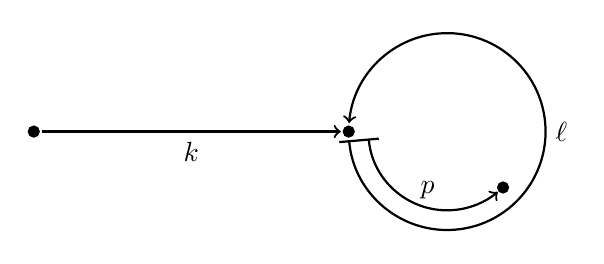
\begin{tikzpicture}
		\filldraw (-2, 0) circle (2pt); % Begin
		\draw[thick, ->] (-1.9, 0) -- node[below] {$k$} (1.9, 0) ;
		\filldraw (2, 0) circle (2pt); % End of k
		\draw[thick, |->] (3.25, 0) ++(-175:1.25) arc (-175:175:1.25);
		\node[xshift=4.7cm] {$\ell$};
		\draw[thick, |->] (3.25, 0) ++(-175:1) arc (-175:-50:1);
		\node[xshift=3cm, yshift=-0.75cm] {$p$};
		\filldraw (3.96, -0.71) circle (2pt);
	\end{tikzpicture}
	
	\caption{A description of how a path can be decomposed into a cycle, the path to it and a last part of it.}
	\label{PathDecompositionPrinciple}
\end{figure}

In the beginning we remarked that we have to fixate an alternation depth.
This bound can be seen in the definition of the transitive expansion and will be used in the logic that will characterise the Colour Refinement algorithm.
Therefore we can only reason about a fragment of $\GFC$, where the terms do not alternate too often.
This is formally stated in the following definition.

\begin{definition}[Alternation bounded $\GFC$]
	The fragment of $\GFC$ with an bounded alternation depth of $k$ ($\GFC_k$) is $\GFC$ with the constraint that for all formulae $\phi\in\GFC_k$ of signature $\sigma$ and every term $t$ that appears in $\phi$, there is an $n\in \mathbb{N}$ and an $\alpha\in \operatorname{Alters}_n^k(\sigma)$ such that $\alpha=t$.
	Atomic formulae are defined as usual, that is, the formulae $R(t_1(x_1),t_2(x_2),\dots,t_n(x_n))$ and $t_1(x_1)=t_2(x_2)$ for terms $t_1,t_2,\dots,t_n$ and variables $x_1,x_2,\dots,x_n$ are atomic formulae.
\end{definition}

With this, we can prove the first result, which allows us to use every $f^m(x)=y$ in a formula.

\begin{lemma}
	Let $\psi(x_1,x_2)\in \GFC_1$ be of the form $f^m(x_1)=x_2$. 
	Then there exists a formula $\theta(x_1,x_2)\in \GFC$ such that for any $\mathfrak A$ with $\Vert \mathfrak A\Vert=n$ it holds
	$$\mathfrak A,a_1,a_2 \models \psi(x_1,x_2) \text{ if, and only if, } \mathfrak A,a_1,a_2 \models \theta(x_1,x_2)$$ 
	and for any $f^{m'}(x)$ that appears in $\theta$ we have $m'\leq n$.
	Furthermore, $\theta(x_1,x_2)$ is of the form $\bigvee \Phi(x_1,x_2)$, and if $\mathfrak A,a_1,a_2\models \theta(x_1,x_2)$, then there is exactly one $\phi(x_1,x_2)\in\Phi$, such that $\mathfrak A,a_1\models \exists^{\geq 1} x_2 . \phi(x_1,x_2)$.
	Additionally, $\theta(x_1,x_2)\in \GFC_1$.
	\label{Simple_fm_to_fk}
\end{lemma}
\begin{proof}
	If $m \leq n$, we let $\theta\coloneqq\psi$ and the claim follows.
	
	Otherwise, we define
	$$\theta(x_1,x_2)\coloneqq \bigvee_{(k,\ell,p)\in \mathcal I(n,m)} \zeta_{(k,\ell,p)}(x_1,x_2)$$
	where
	\begin{align*}
		\zeta_{(k,\ell,p)}(x_1,x_2)\coloneqq & f^{k+p}(x_1)=x_2 \land f^{k}(x_1)=f^{k+\ell}(x_1) \\
		& \land \operatorname{E}^{k,\ell}_{f}(x_1)  \\
		& \land \bigwedge_{\ell'<\ell}f^{k}(x_1)\neq f^{k+\ell'}(x_1)
	\end{align*}
	and for some term $t(x_1)$ we have
	$$\operatorname{E}^{k,\ell}_{f}(t(x_1))=\begin{cases}
		\top & \text{if } k=0 \\
		f^{k-1}(t(x_1))\neq f^{k-1+\ell}(t(x_1)) & \text{otherwise}.
	\end{cases}$$
	Due to the definition of $\mathcal I(n,m)$ it is obvious that only $f^{m'}$ with $m'\leq n$ appears.
	We now proceed to the proof of the equivalence.
	For the purpose of readability, we will write $f_{\mathfrak A}$ instead of $f^{\mathfrak A}$.
	
	We will show that if $\mathfrak A,a_1,a_2 \models \theta(x_1,x_2)$, then $\mathfrak A,a_1,a_2 \models \psi(x_1,x_2)$.
	Let $\mathfrak A,a_1,a_2 \models \theta(x_1,x_2)$. 
	By definition of $\theta$, there are $(k,\ell,p)\in \mathcal I(n,m)$ with $\mathfrak A,a_1,a_2 \models \zeta_{(k,\ell,p)}(x_1,x_2)$.
	In particular $f_{\mathfrak A}^{k}(a_1)=f_{\mathfrak A}^{k+\ell}(a_1)$. It follows that
	$$f_{\mathfrak A}^{k}(a_1)=f_{\mathfrak A}^{k+\ell}(a_1)=f_{\mathfrak A}^{k+2\ell}(a_1)=f_{\mathfrak A}^{k+3\ell}(a_1) = \dots = f_{\mathfrak A}^{k+r\cdot \ell}(a_1)$$
	for all $r\in \mathbb N$. By using the definition of $\mathcal{I}(n,m)$, we get
	$$a_2 =f_{\mathfrak A}^{k+p}(a_1) = f_{\mathfrak A}^{k+r\cdot \ell + p}(a_1)=f_{\mathfrak A}^{m}(a_1).$$
	From this we can deduce $\mathfrak A,a_1,a_2\models \psi(x_1,x_2)$, where $\psi(x_1,x_2)$ has the form $f^{m}(x_1)=x_2$.
	
	Now we prove that if $\mathfrak A,a_1,a_2 \models \psi(x_1,x_2)$, then $\mathfrak A,a_1,a_2 \models \theta(x_1,x_2)$. 
	Let $\mathfrak A,a_1,a_2\models \psi(x_1,x_2)$. By assumption $m>n$ and by the pigeonhole principle there have to be distinct $i$ and $j$ such that $f_{\mathfrak A}^{i}(a_1)=f_{\mathfrak A}^{j}(a_1)$.
	Choose such $i$, $j$ such that they are lexicographically minimal.
	Now choose $k\coloneqq i$, $\ell \coloneqq j-i$ and $p\coloneqq (m-i) \mod (j-i)= (m-i) \mod \ell$.
	Obviously $(k,\ell,p)\in\mathcal I(n,m)$ and what remains to be shown is that $\mathfrak A,a_1,a_2\models \zeta_{(k,\ell,p)}(x_1,x_2)$.
	For that, we consider the parts of the conjunction and show for each one that it is satisfied.
	
	\begin{itemize}
		\item $f^{k+p}(x_1)=x_2$ is satisfied.
		We use the fact that $a= b \mod c \Leftrightarrow b = r\cdot c +a \text{ for some } r\in \mathbb N$.
		Then
		$$f_{\mathfrak A}^{k+p}(a_1)=f_{\mathfrak A}^{i+(m-i)-r\cdot \ell}(a_1)=f_{\mathfrak A}^{i+r\cdot \ell + m -i - r\cdot \ell}(a_1)=f_{\mathfrak A}^{m}(a_1)=a_2.$$
		Therefore $\mathfrak A,a_1,a_2\models f^{k+p}(x_1)=x_2$.
		
		\item $f^{k}(x_1)=f^{k+\ell}(x_1)$ is satisfied.
		Consider that
		$$f_{\mathfrak A}^{k}(a_1)=f_{\mathfrak A}^{i}(a_1)=f_{\mathfrak A}^{j}(a_1)=f_{\mathfrak A}^{j+i-i}(a_1)=f_{\mathfrak A}^{i+j-i}(a_1)=f_{\mathfrak A}^{k+\ell}(a_1).$$
		This leads to $\mathfrak A,a_1,a_2\models f^{k}(x_1)=f^{k+\ell}(x_1)$.
		
		\item $\operatorname{E}^{k,\ell}_f(x_1)$ is satisfied.
		Otherwise $f_{\mathfrak A}^{k-1}(a_1)=f_{\mathfrak A}^{k-1+\ell}(a)$, but then $(k-1,\ell)$ would be lexicographically smaller than $(i,j)$.
		
		\item The same reasoning applies to $\bigwedge_{\ell'<\ell}f^{k}(x_1)\neq f^{k+\ell'}(x_1)$. 
		If it weren't satisfied, there would be a $(i,j')$ with $j'<j$ and $f_{\mathfrak A}^{i}(a_1)=f_{\mathfrak A}^{i+j'}(a_1)$ which would be lexicographically smaller than $(i,j)$.
	\end{itemize}
	
	Thus we have shown that every subformula of the conjunction and therefore the formula is being fulfilled.
	
	Lastly, it remains to prove that if $\theta$ is satisfied, then there is exactly one $(k,\ell,p)\in\mathcal{I}(n,m)$ such that $\exists^{\geq 1}x_2.\zeta_{(k,\ell,p)}(x_1, x_2)$ is fulfilled.
	We prove this by contradiction.
	Assume that $\mathfrak A,a_1,a_2\models \theta(x_1,x_2)$ and that there are $\zeta_{(k,\ell,p)}(x_1,x_2)$ and $\zeta_{(k',\ell',p')}(x_1,x_2)$ with $(k,\ell,p)\neq (k',\ell',p')$, such that $\mathfrak A,a_1\models \exists^{\geq 1}x_2.\zeta_{(k,\ell,p)}(x_1,x_2)$ and $\mathfrak A,a_1\models \exists^{\geq 1}x_2.\zeta_{(k',\ell',p')}(x_1,x_2)$.
	
	We proceed with a case distinction. 
	Let $k=k'$ and $\ell=\ell'$.
	Then there are $r,r'\in\mathbb N$ such that
	$$k+r\cdot \ell + p = k'+r'\cdot \ell' + p'=m.$$
	Thus we can infer that $r\cdot \ell+p = r'\cdot \ell'+p'$.
	By definition of $\mathcal{I}(n,m)$ we know that $p,p'<\ell=\ell'$ and as such 
	$$r\cdot \ell +p,r'\cdot \ell'+p'\in \{r\cdot \ell,r\cdot \ell +1,\dots, r\cdot \ell +(\ell-1)\}$$
	and because $p$ is a non-negative integer, $r=r'$ has to follow and further we get $p=p'$.
	However this would contradict that $(k,\ell,p)\neq (k',\ell',p')$.
	Now assume that $\ell\neq\ell'$ and without loss of generality assume that $\ell<\ell'$.
	But then $\mathfrak A,a_1 \not\models \bigwedge_{\hat{\ell}<\ell'}f^{k'}(x_1)\neq f^{k'+\hat{\ell}}(x_1)$, because 
	$$f^{k'+\ell}_{\mathfrak A}(a_1)=f^{k+\ell}_{\mathfrak A}=f^k_{\mathfrak A}(a_1)=f^{k'}_{\mathfrak A}(a_1)$$
	and $k'+\ell < k'+\ell'$.
	Thus this cannot be the case as well.
	
	Consider that $k\neq k'$ and without loss of generality assume that $k<k'$.
	If $\ell=\ell'$, then by the principle of induction, we get that $f_{\mathfrak A}^k(a_1)=f_{\mathfrak A}^{k+\ell}(a_1)$, $f_{\mathfrak A}^{k+1}(a_1)=f_{\mathfrak A}^{k+1+\ell}(a_1)$ and then $f_{\mathfrak A}^{k'}(a_1)=f_{\mathfrak A}^{k'+\ell'}(a_1)$.
	But this contradicts $\mathfrak A,a_1 \models \operatorname{E}^{k',\ell'}_f(x_1)$.
	If $\ell < \ell'$, then 
	$$f_{\mathfrak A}^{k'}(a_1) =f_{\mathfrak A}^{k+(k'-k)}(a_1)=f_{\mathfrak A}^{k+(k'-k)+\ell}(a_1) = f_{\mathfrak A}^{k'+\ell}(a_1),$$
	but this again contradicts $\mathfrak A,a_1 \models \bigwedge_{\hat{\ell}<\ell'}f^{k'}(x_1)\neq f^{k'+\hat{\ell}}(x_1)$.
	If $\ell'<\ell$, then there exists a $t\in\mathbb N$ such that 
	$$k+t\cdot  \ell < k' \leq k+(t+1)\cdot \ell.$$
	We now define $r\coloneqq k+(t+1)\cdot \ell -k'$ and get $f_{\mathfrak A}^{k'+r}(a_1)=f_{\mathfrak A}^{k'+r+\ell'}$ and by using $f_{\mathfrak A}^{k'+r}(a_1)=f_{\mathfrak A}^{k+(t+1)\cdot \ell}(a_1)=f_{\mathfrak A}^k(a_1)$ it follows that $f_{\mathfrak A}^{k}(a_1)=f_{\mathfrak A}^{k+\ell'}(a_1)$.
	This contradicts $\mathfrak A,a_1 \models \bigwedge_{\hat{\ell}<\ell}f^{k}(x_1)\neq f^{k'+\hat{\ell}}(x_1)$.
	
	One can see that we did not use $x_2$ or $a_2$.
	Therefore its interpretation is irrelevant, which is why we can existentially quantify it in the claim.
	As all possible cases lead to a contradiction, the first assumption cannot be true and we proved the claim.
	
	As we did not use any function symbols other than $f$, $\theta(x_1,x_2)\in \GFC_1$ follows obviously.
\end{proof}

The above proof allows for the translation of a formula $f^m(x)=y$ to a formula $\theta(x,y)$ that is equivalent for structures with $n$ elements.
A natural extension would be, to allow alternation of functions, for example formulae like $g^m(f^{m'}(x))=y$.
This is also possible and will be proved in the following.

\begin{lemma}
	Let $d\in\mathbb d$ and $\psi(x_1,x_2)\in \GFC_d$ be of the form $t(x_1)=x_2$ for a term $t$.
	Then there exists a formula $\theta_{t}(x_1,x_2)\in\GFC_d$, such that for any structure $\mathfrak A$ with $\Vert \mathfrak A \Vert = n$ it holds
	$$\mathfrak A,a_1,a_2 \models \psi(x_1,x_2) \text{ if, and only if, } \mathfrak A,a_1,a_2 \models \vartheta_{t}(x_1,x_2).$$ 
	Furthermore, $\theta_{t}(x_1,x_2)$ is of the form $\bigvee \Phi(x_1,x_2)$ where all $\phi(x_1,x_2)\in\Phi(x_1,x_2)$ are of the form
	$$t'(x_1)=x_2 \land \bigwedge \Psi(x_1)$$ 
	for some term $t'(x_1)$, and for every function symbol $f$ in the signature, there does not appear a term of the form $f^m(s(x))$ where $m > n$.
	Additionally, if $\mathfrak A,a_1,a_2\models \theta_{t}(x_1,x_2)$, then there is exactly one $\phi\in\Phi$, such that $\mathfrak A,a_1\models \exists^{\geq 1}x_2.\phi(x_1,x_2)$.
	\label{TranslationOfArbTerms}
\end{lemma}
\begin{proof}
	We prove this via an induction on the term $t(x_1)$.
	
	\textbf{Base case:}
	If $t(x_1)$ is of the form $f^{m}(x_1)$ for a unary function symbol $f$ and $m\in \mathbb N$, we use the formula constructed in the proof of \cref{Simple_fm_to_fk}.
	It can easily be verified that it is in the correct form and from the same proof we get that if the translated formula is fulfilled, exactly one subformula of the disjunction is satisfied.
	
	\textbf{Inductive step:}
	Assume that $t(x_1)$ is of the form $g^m(s(x_1))$ for a unary function symbol $g$, $m\in\mathbb N$ and term $s$.
	By the induction hypothesis, there is a formula $\theta_{s}(x_1,x_2)\in \GFC_{d-1}$ of the form $\bigvee \Phi_s(x_1,x_2)$ defined above with $\mathfrak A,a_1,a_2 \models s(x_1)=x_2$ if, and only if, $\mathfrak A,a_1,a_2\models \theta_{s}(x_1,x_2)$.
	
	If $m\leq n$, we set $\theta_{t}(x_1,x_2)$ to
	$$\bigvee \Phi'(x_1,x_2),$$
	where $\Phi'(x_1,x_2)\coloneqq\{g^{m}(t'(x_1))=x_2 \land \bigwedge \Psi(x_1) : t'(x_1)=x_2 \land \bigwedge \Psi(x_1)\in \Phi_s(x_1,x_2)\}$.
	
	If $m>n$, then we set $\theta_{t}(x_1,x_2)$ to
	$$\bigvee_{(k,\ell,p)\in \mathcal I(n,m)} \bigvee \Phi'_{(k,\ell,p)}(x_1,x_2),$$
	where 
	\begin{align*}
		\Phi'_{(k,\ell,p)}\coloneqq \{g^{k+p}(t'(x_1))=x_2 &\land g^{k}(t'(x_1))=g^{k+l}(t'(x_1)) \\
		& \land \operatorname{E}^{k,l}_g(t'(x_1)) \land \bigwedge_{\ell'<\ell} g^{k}(t'(x_1))\neq g^{k+\ell'}(t'(x_1)) \\
		& \land \Psi(x_1) : t'(x_1)=x_2 \land \bigwedge \Psi(x_1)\in \Phi_s(x_1,x_2)\}
	\end{align*}
	
	By using the above definitions, we get $\mathfrak A,a_1,a_2\models s(x_1)=x_2$ if, and only if, $\mathfrak A,a_1,a_2\models \phi_s(x_1,x_2)$ for some $\phi_s\in\Phi_s$ where $\phi_s(x_1,x_2)$ is of the form $t'(x_1)=x_2 \land \bigwedge \Psi(x_1)$.
	Therefore
	\begin{equation}
		\mathfrak A, a_1,a_2 \models s(x_1)=x_2 \text{ if, and only if, } \mathfrak A,a_1,a_2 \models t'(x_1)=x_2 \land \bigwedge \Psi(x_1).
		\label{Equivalence_s_and_tPsi}
	\end{equation}
	
	We now prove that 
	$$\mathfrak A, a_1,a_2\models t(x_1)=x_2 \text{ if, and only if, } \mathfrak A,a_1,a_2\models \theta_{t}(x_1,x_2).$$
	Assume $m\leq n$.
	Let $\mathfrak A, a_1,a_2 \models \theta_{t}$.
	Then there is some $\phi(x_1,x_2)$ of the form $g^{m}(t'(x_1))=x_2 \land \bigwedge \Psi(x_1)$ such that $\mathfrak A,a_1,a_2\models \phi(x_1,x_2)$.
	We then get
	\begin{align*}
		\mathfrak A,a_1,a_2 \models & g^{m}(t'(x_1))=x_2 \land \bigwedge \Psi(x_1) \\
		\Leftrightarrow \mathfrak A,a_1,a_2,a_3 \models & g^{m}(x_3)=x_2 \land \bigwedge \Psi(x_1) \land t'(x_1)=x_3 \text{ for some } a_3\in A \\
		\overset{(\ref{Equivalence_s_and_tPsi})}{\Leftrightarrow} \mathfrak A,a_1,a_2,a_3\models & g^{m}(x_3)=x_2 \land s(x_1)=x_3 \text{ for some } a_3\in A \\
		\Leftrightarrow \mathfrak A,a_1,a_2 \models & g^{m}(s(x_1))=x_2.
	\end{align*}
	
	Now let $m>n$.
	Then there is a
	\begin{align*}
		\phi(x_1,x_2)\coloneqq g^{k+p}(t'(x_1))=x_2 &\land g^{k}(t'(x_1))=g^{k+l}(t'(x_1)) \\
		& \land \operatorname{E}^{k,l}_g(t'(x_1)) \land \bigwedge_{\ell'<\ell} g^{k}(t'(x_1))\neq g^{k+\ell'}(t'(x_1)) \\
		& \land \bigwedge \Psi(x_1)
	\end{align*}
	for some $(k,\ell,p)\in\mathcal I(n,m)$ with $\mathfrak A,a_1,a_2\models \phi(x_1,x_2)$.
	And now
	\begin{align*}
		\mathfrak A,a_1,a_2 \models & \phi(x_1,x_2) \\
		\Leftrightarrow A,a_1,a_2,a_3 \models &g^{k+p}(x_3)=x_2 \land g^{k}(x_3)=g^{k+l}(x_3) \\
		& \land \operatorname{E}^{k,l}_g(x_3) \land \bigwedge_{\ell'<\ell} g^{k}(x_3)\neq g^{k+\ell'}(x_3) \\
		& \land \bigwedge\Psi(x_1) \land t'(x_1)=x_3 \text{ for some } a_3\in A \\
		\overset{\cref{Simple_fm_to_fk}}{\Leftrightarrow} \mathfrak A, a_1,a_2,a_3 \models & g^{m}(x_3)=x_2 \land t'(x_1)=x_3 \land \bigwedge\Psi(x_1) \text{ for some } a_3 \in A \\
		\overset{\cref{Equivalence_s_and_tPsi}}{\Leftrightarrow} \mathfrak A,a_1,a_2,a_3 \models & g^{m}(x_3)=x_2\land s(x_1)=x_3 \text{ for some } a_3\in A \\
		\Leftrightarrow \mathfrak A,a_1,a_2 \models & g^{m}(s(x_1))=x_2.
	\end{align*}
	The other direction follows in both cases, as only equivalent steps have been used and it is obvious that the disjunction of a set is being fulfilled, if a formula of the set is satisfied.
	
	Lastly, we show that if $\mathfrak A,a_1,a_2\models \theta_t(x_1,x_2)$, where $\theta_t$ is of the form $\bigvee \Phi$, there is exactly one $\phi\in\Phi$, such that $\mathfrak A,a_1\models \exists^{\geq 1} x_2.\phi(x_1,x_2)$.
	As in the proof of \cref{Simple_fm_to_fk}, we are going to use a proof by contradiction and we will look at the cases where $m\leq n$ and $m> n$ separately.
	If $m\leq n$, assume that $\mathfrak A,a_1,a_2\models \theta_t(x_1,x_2)$ and that there are $\phi_1,\phi_2\in \Phi'(x_1,x_2)$ with $\phi_1\neq \phi_2$, $\mathfrak A,a_1\models \exists^{\geq 1}x_2.\phi_1(x_1,x_2)$ and $\mathfrak A,a_1\models \exists^{\geq 1}x_2.\phi_2(x_1,x_2)$.
	It is easy to see that 
	$$\mathfrak A,a_1,a_2\models g^m(t'_1(x_1))=x_2 \land \bigwedge \Psi_1(x_1) \land g^m(t'_2(x_1))=x_2 \land \bigwedge\Psi_2(x_1)$$
	for some $a_2$, which is equivalent to
	$$\mathfrak A,a_1,a_2,a_3,a_4\models g^m(x_3)=x_2 \land t'_1(x_1)=x_3\land \Psi_1(x_1) \land g^m(x_4)=x_2 \land t'_2(x_1)=x_4 \land \Psi_2(x_1)$$
	when using the correct $a_3$ and $a_4$.
	However, $t'_1(x_1)=x_2\land \Psi_1(x_1), t'_2(x_1)=x_s \land \Psi_2(x_1) \in \Phi_s$ and thus there would be $\psi_1(x_1,x_3/x_2),\psi_2(x_1,x_4/x_2) \in \Phi_s$, such that $\mathfrak A,a_1\models \exists^{\geq 1}x_3. \psi(x_1,x_3)$ and $\mathfrak A,a_1\models \exists^{\geq 1}x_4.\psi(x_1,x_4)$.
	This is a contradiction to the induction hypothesis.
	
	If $m>n$, we again assume that $\mathfrak A,a_1,a_2\models \theta_t(x_1,x_2)$ and that there are $\phi_1(x_1,x_2)\in\Phi'_{(k,\ell,p)}(x_1,x_2)$ and $\phi_2(x_1,x_2)\in\Phi'_{(k',\ell',p')}(x_1,x_2)$ with $\phi_1\neq \phi_2$, $\mathfrak A,a_1\models \exists^{\geq 1}x_2.\phi_1(x_1,x_2)$ and $\mathfrak A,a_1\models \exists^{\geq 1}x_2.\phi_2(x_1,x_2)$.
	By looking at the structure of the formulae as they are defined in this proof and by substituting terms and variables like in the first case, we again find that 
	$$\mathfrak A,a_1,a_3,a_4\models t'_1(x_1)=x_3\land \Psi_1(x_1) \land t'_2(x_1)=x_4 \land \Psi_2(x_1),$$
	where $t'_1(x_1)=x_2\land\bigwedge \Psi_1(x_1), t'_2(x_1)=x_2\land\bigwedge \Psi_2(x_1)\in \Phi_2$.
	By using the same arguments as before, we as well arrive at a contradiction.
	As such, the assumption must be false and we have finished the proof.
\end{proof}

A corollary of the above lemma is that the same statement also holds for an arbitrary relation, in addition to equality.

\begin{lemma}
	Let $d\in\mathbb N$ and $\psi(x_1,\dots,x_m)\coloneqq R(t_1(x_1),\dots,t_m(x_m))\in \GFC_d$ be an atomic formula.
	Then there exists a formula $\theta_\psi\in\GFC_d$, such that for any given structure (of fitting signature) $\mathfrak A$ with $\Vert\mathfrak A \Vert=n$ it holds
	$$\mathfrak A,a_1,\dots,a_m\models \psi(x_1,\dots,x_m) \text{ if, and only if, } \mathfrak A,a_1,\dots,a_m\models \theta_\psi(x_1,\dots,x_m).$$
	Furthermore, $\theta_\psi(x_1,\dots,x_m)$ is of the form $\bigvee \Phi(x_1,\dots,x_m)$ where all $\phi\in\Phi$ are of the form
	$$R(t_1'(x_1),\dots,t_m'(x_m))\land \bigwedge\Psi_1(x_1)\land \dots\land\bigwedge \Psi_m(x_m),$$
	and for every $f^m(s(x))$ that appear in $\theta_\psi$, where $f$ is a unary function symbol and $s$ is a term, $m\leq n$.
	Additionally, if $\mathfrak A,a_1,\dots,a_,\models \theta_\psi(x_1,\dots,x_m)$, then there exists exactly one $\phi(x_1,\dots,x_m)\in\Phi(x_1,\dots,x_m)$, such that $\mathfrak A,a_1,\dots,a_m\models \phi(x_1,\dots,x_m)$.
	\label{TranslationOfArbAtomics}
\end{lemma}
\begin{proof}
	Let $\mathfrak A,a_1,\dots,a_m\models\psi(x_1,\dots,x_m)$.
	This is equivalent to 
	$$\mathfrak A,a_1,\dots,a_m,b_1,\dots,b_m\models R(b_1,\dots,b_m)\land t_1(x_1)=b_1\land\dots\land t_m(x_m)=b_m$$
	for some $b_1,\dots,b_m\in A$.
	By applying the previous lemma, we get the equivalent statement
	\begin{align*}
		\mathfrak A,a_1,\dots,a_m,b_1,\dots,b_m\models R(y_1,\dots,y_m) \land& \bigvee_{i_1}\left(t_{1,i_1}'(x_1)=y_1\land \bigwedge\Psi_{1,i_1}(x_1)\right) \\
		\land& \dots \\
		\land& \bigvee_{i_m}\left(t_{m,i_m}'(x_m)=y_m\land \bigwedge\Psi_{m,i_m}(x_m)\right).
	\end{align*}
	Through distribution of boolean formulae we get
	\begin{align}
		\mathfrak A,a_1,\dots,a_m,b_1,\dots,b_m\models \bigvee_{i_1} \dots \bigvee_{i_m} ( R(y_1,\dots,y_m)\land & t_{1,i_1}'(x_1)=y_1 \land \bigwedge\Psi_{1,i_1}(x_1) \nonumber \\
		\land & \dots \label{EquivalentDistributedAtomic}\\
		\land & t_{m,i_m}'(x_m)=y_m \land \bigwedge\Psi_{m,i_m}(x_m) ). \nonumber
	\end{align}
	Finally, we can resubstitute variables and get
	\begin{align*}
		\mathfrak A,a_1,\dots,a_m\models \bigvee_{i_1}\dots\bigvee_{i_m} &(R(t_{1,i_1}'(x_1),\dots,t_{m,i_m}'(x_m)) \\
		&\land \bigwedge\Psi_{1,i_1}(x_1) \\
		&\land\dots \\
		&\land\bigwedge\Psi_{m,i_m}(x_m))\eqqcolon \theta_\psi(x_1,\dots,x_m).
	\end{align*}
	One can see that $\theta_\psi$ is of the correct form.
	The equality follows from the fact that only equivalences have been used to derive $\theta_\psi$ from $\psi$.
	
	Lastly, we prove that if $\theta_\psi$ is satisfied, there is exactly one formula of the disjunction that is satisfied.
	For this, consider the equivalent formula from \cref{EquivalentDistributedAtomic}.
	Assume that $\mathfrak A,a_1,\dots,a_m\models \theta_\psi$ and that there are two subformulae $\phi_1$ and $\phi_2$ of the formula in \cref{EquivalentDistributedAtomic}, where $\phi_1$ is of the form 
	\begin{align*}
		R(y_1,\dots,y_m)\land & t_{1,i_1}'(x_1)=y_1 \land \bigwedge\Psi_{1,i_1}(x_1) \\
		\land & \dots \\
		\land & t_{m,i_m}'(x_m)=y_m \land \bigwedge\Psi_{m,i_m}(x_m)
	\end{align*}
	and $\phi_2$ is of the form
	\begin{align*}
		R(y_1,\dots,y_m)\land & s_{1,i_1}'(x_1)=y_1 \land \bigwedge\Psi'_{1,i_1}(x_1) \\
		\land & \dots \\
		\land & s_{m,i_m}'(x_m)=y_m \land \bigwedge\Psi'_{m,i_m}(x_m),
	\end{align*}
	such that $\phi_1\neq\phi_2$, $\mathfrak A,a_1,\dots,a_m,b_1,\dots,b_m\models \phi_1$ and $\mathfrak A,a_1,\dots,a_m,b_1,\dots,b_m\models \phi_2$.
	As $\phi_1\neq \phi_2$, there must be a $j$ such that $\psi_1$ is of the form $t'_{j,i_j}(x_j)=y_j\land \bigwedge \Psi_{j,i_j}(x_j)$, $\psi_2$ is of the form $s'_{j,i_j}(x_j)=y_j\land\bigwedge \Psi'_{j,i_j}(x_j)$ and $\psi_1\neq\psi_2$.
	From the construction of the formula we know, that there is a term $t_j$, a formula $\theta_{t_j}$ of the form $\bigvee \Phi_{t_j}$ and $\psi_1,\psi_2\in\Phi_{t_j}$.
	However, $\mathfrak A,a_j\models \exists^{\geq 1}y_j . \psi_1(x_j,y_j)$ and $\mathfrak A,a_j\models \exists^{\geq 1}y_j.\psi_2(x_j,y_j)$ would contradict the claim that has been proved in \cref{TranslationOfArbTerms}.
\end{proof}

To illustrate how this translation works, let us consider the formula $\psi$ of the form $g^4(f^3(x))=y$ for a structure with $2$ elements.
As in the proof, we inductively translate the inner terms and as such get for the formula $f^3(x)=y$, the formula $\phi$ of the form
$$\bigvee_{(k,\ell,p)\in \mathcal I(2,3)}\left(f^k(x)=f^{k+\ell}(x)\land f^{k+p}(x)=y \land \operatorname{E}^{k,l}_f(x)\land\bigwedge_{\hat \ell < \ell} f^k(x)\neq f^{k+\hat\ell}(x)\right)$$
and with $\mathcal I(2,3)=\{(0,2,1),(1,1,0),(0,1,0)\}$ we get that $\phi$ equals
\begin{align*}
	\phantom{\lor}&\left(x=f^2(x) \land f(x)=y \land x\neq f(x)\right) \\
	\lor & \left(f(x)=f^2(x) \land f(x)=y \land x \neq f(x)\right) \\
	\lor & \left(x=f(x) \land x=y \land \top\right).
\end{align*}
Now we can construct $\theta_\psi$ from $\psi$. 
From the proof, we know that $\theta_\psi$ is of the form
\begin{align*}
	\bigvee_{(k',\ell',p')\in \mathcal I(2,4)}\bigvee_{(k,\ell,p)\in \mathcal I(2,3)} ( &f^k(x)=f^{k+\ell}(x)\land \operatorname{E}^{k,l}_f(x)\land\bigwedge_{\hat{\ell}<\ell}f^k(x)\neq f^{k+\hat\ell}(x) \\
	\land & g^{k'}(f^{k+p}(x))=g^{k'+\ell'}(f^{k+p}(x)) \land g^{k'+p'}(f^{k+p}(x)) = y \\
	\land & E^{k',\ell'}_g(f^{k+p}(x)) \land \bigwedge_{\hat{\ell}<\ell'}g^{k'}(f^{k+p}(x))\neq g^{k'+\hat\ell}(f^{k+p}(x))
\end{align*}
and with $\mathcal I(2,4)=\{(1,1,0),(0,1,0), (0,2,0)\}$ we can analogous find that $\theta_\psi$ is equal to
\todo{Das ist ja eine Disjunktion mit 3*3=9 Formeln die jeweils etwa eine Zeile lang sind. Sollte ich die trotzdem komplett aufschreiben?}

This now allows us to proof the logical characterisation of our Colour Refinement Algorithm.

\begin{theorem}
	\label{thm:ThmB}
	Let $\mathfrak A$ and $\mathfrak B$ be two structures of the same signature $\sigma$ with relation and unary function symbols and let $k\in \mathbb{N}$
	The two following statements are equivalent:
	\begin{enumerate}
		\item $\RCR_k$ distinguishes $\mathfrak A$ and $\mathfrak B$.
		\item There exists a sentence $\phi\in\GFC_k$ such that $\mathfrak A\models \phi$ and $\mathfrak B\not\models \phi$.
	\end{enumerate}
\end{theorem}
\begin{proof}
	We prove that \emph{1.} implies \emph{2.}. 
	Let $\mathfrak A$ and $\mathfrak B$ be distinguished by $\RCR_k$.
	If they are of different sizes, assume without loss of generality that 
	$$\Vert \mathfrak A \Vert =n > n'=\Vert \mathfrak B \Vert.$$
	Then define $\phi\coloneqq \exists^{\geq n} x. \top\in \GFC_k$, which obviously distinguishes the structures.
	
	Now assume $\Vert \mathfrak A\Vert = \Vert \mathfrak B \Vert = n$.
	By definition, $\RCR$ distinguishes $\widetilde{\mathfrak A}$ and $\widetilde{\mathfrak B}$.
	When using the proof from \cite{scheidt2025ColorRefinement}, we obtain a formula $\widetilde{\phi}\in \GFC$ of signature $\widetilde{\sigma}$ that distinguishes the expansions.
	This formula $\widetilde{\phi}$ can then be translated to a formula $\phi\in\GFC_k$ of signature $\sigma$.
	For every atomic subformula $\operatorname{Eq}_{\alpha,\beta}(x,y)$, where $\alpha,\beta\in \operatorname{Alters}_n^k(\sigma)$, replace it by the formula $\alpha(x)=\beta(y)$,
	and every atomic subformula $R_{\alpha_1,\dots,\alpha_\ell}(x_1,\dots,x_\ell)$, replace it by the formula $R(\alpha_1(x_1),\dots,\alpha_\ell(x_\ell))$.
	Obviously, if a structure's expansion satisfied $\widetilde{\phi}$, it also satisfies $\phi$ and vice versa.
	Therefore, we get a formula $\phi\in \GFC_k$ that distinguishes $\mathfrak A$ and $\mathfrak B$.
	
	Now we prove that \emph{2.} implies \emph{1.}.
	Let $\phi\in \GFC_k$ such that $\mathfrak A\models \phi$ and $\mathfrak B\not\models \phi$.
	Using \cref{TranslationOfArbAtomics} we can obtain a formula $\theta_\psi$ for every atomic subformula $\psi$ of $\phi$ with $\mathfrak A\models \psi$ if, and only if, $\mathfrak A\models \theta_\psi$.
	With this we can construct an equivalent formula $\phi'\in\GFC_k$, which then allows us, to easily translate it to $\widetilde{\sigma}$.
	We will construct this formula $\phi'$ inductively and directly prove the equivalence.
	
	\begin{claim}
		The two formulae $\phi$ and $\phi'$ are equivalent.
	\end{claim}
	\begin{proof}
		\textbf{Base cases:}
		If $\phi$ is an atomic formula, that is, either a term equivalence or a relation, then set $\phi'$ to $\theta_\phi$.
		The equivalence follows directly from the above lemmas \ref{TranslationOfArbTerms} and \ref{TranslationOfArbAtomics}.
		
		\textbf{Inductive cases:}
		In the cases where $\phi$ is of the form $\neg\theta$ or $\theta_1\land\theta_2$, we set $\phi'$ to $\neg\theta'$ or $\theta_1'\land\theta_2'$ and the claim follows directly using the induction hypothesis.
		
		Let $\phi$ be of the form $\exists^{\geq\ell}\mathbf v. \Delta\land \theta$.
		In addition to translating $\Delta$ and $\theta$ to $\theta_\Delta$ and $\theta'$ respectively, we also will need to transform the formula, so that it still is a valid formula in $\GFC_k$.
		When looking at the possible translations from the atomic formula $\Delta(x_1,\dots,x_m)$, we see that it must be of the form $\bigvee_{i\in[o]} (\Delta'_i(x_1,\dots,x_m) \land \bigwedge \Psi_i(x_1,\dots,x_m))$.
		When considering the transformed formula 
		$$\exists^{\geq \ell}\mathbf v. \left(\bigvee_{i\in [o]}(\Delta'_i\land\bigwedge \Psi_i) \land \theta'\right),$$
		we then will distribute $\theta$ over the disjunction and thus define
		$$\psi \coloneqq \exists^{\geq \ell}\mathbf v. \left(\bigvee_{i\in[o]} \Delta'_i\land\bigwedge \Psi_i \land \theta'\right)$$
		In the following we prove the equivalence of $\phi$ and $\psi$.
		Let $\mathfrak A\models \phi$.
		This means there are at least $\ell$ tuples $\mathbf a\in A$, such that $(\mathfrak A,\mathbf a)\models \Delta(\mathbf v) \land \theta(\mathbf v)$.
		Using the induction hypothesis we get that this is equivalent to $(\mathfrak A,\mathbf a)\models \bigvee(\Delta'\land\bigwedge\Psi)\land \theta'$, which, using the distributive law of propositional logic, is equivalent to $(\mathfrak A,\mathbf a)\models \bigvee(\Delta'\land\bigwedge\Psi\land\theta')$.
		Therefore the number of tuples that satisfy $\Delta\land\theta$ must be the same as for $\bigvee(\Delta'\land\bigwedge\Psi\land\theta')$ and $\mathfrak A\models \exists^{\geq\ell}\mathbf v. \bigvee (\Delta'\land\bigwedge\Psi\land\theta')$ follows.
		
		However, we are not finished, because $\psi \notin \GFC_k$.
		We will solve this, by considering all possible segmentations of the disjunction.
		Formally, for $o,n\in\mathbb N$ we define $\operatorname{Parts}(o, n)$ as the set of all multisets with exactly $n$ elements of $[o]$, respecting their multiplicity.
		We then define $\phi'$ as
		$$\bigvee_{(M,\operatorname{mult}_M)\in \operatorname{Parts}(o,\ell)} \bigwedge_{i\in M} \exists^{\geq \operatorname{mult}_M(i)}\mathbf v. (\Delta'_i\land\bigwedge \Psi_i \land \theta')$$
		and will prove the equivalence between $\psi$ and $\phi'$ in the following. 
		
		Let $\mathfrak A\models \psi$.
		Then there are $\ell$ different tuples $\mathbf a$, such that $\mathfrak A,\mathbf a \models \bigvee_{i\in[o]}(\Delta'_i\land\bigwedge\Psi_i\land\theta')$.
		From the above lemmas we know that for every such tuple, there is exactly one $i$ such that $\mathfrak A,\mathbf a\models \Delta'_i\land\bigwedge \Psi_i\land \theta'$.
		Now construct a multiset $(M,\operatorname{mult}_M)$ with exactly these $i$ that are being satisfied and with the multiplicity of the amount of tuples satisfying them.
		One can see that $(M,\operatorname{mult}_M)\in \operatorname{Parts}(o,n)$ and that 
		$$\mathfrak A \models \bigwedge_{i\in M}\exists^{\geq\operatorname{mult}_M(i)}\mathbf v. (\Delta'_i\land \bigwedge\Psi_i\land \theta').$$
		It directly follows that $\mathfrak A\models \phi'$.
		
		Let $\mathfrak A\models \phi'$.
		From the construction we know, that every $\mathbf a$ that is being quantified satisfies only the $\Delta'_i\land\bigwedge\Psi_i\land\theta'$ they are being quantified for.
		By the definition of $\operatorname{Parts}(o,\ell)$, we thus get exactly $\ell$ tuples that satisfy some $\Delta'_i\land\bigwedge\Psi_i\land\theta'$ and $\mathfrak A\models \psi$ follows.
	\end{proof}
	
	Note that for every term $\alpha$ that appears in $\phi'$, it holds that $\alpha\in \operatorname{Alters}^k_n(\sigma)$.
	This follows from the properties of the translation in \cref{TranslationOfArbAtomics}.
	Furthermore, for every atomic subformula, we have a corresponding relation symbol in $\widetilde{\sigma}$.
	With this, we can transform $\phi'$ to a formula $\widetilde{\sigma}\in\GFC$ of signature $\widetilde{\sigma}$, such that $\mathfrak A\models \phi'$ if, and only if, $\widetilde{\mathfrak A}\models \widetilde{\phi}$.
	
	It can be seen that the only subformulae that need to be changed are atomic.
	Let $\psi$ be an atomic formula that appears in $\phi'$.
	If $\psi$ is a term equation, that is, it is of the form $t(x)=s(y)$, we know through the construction of $\phi'$ and the definition of the transitive expansion, that there are $\alpha,\beta\in \operatorname{Alters}^k_n(\sigma)$ with $\alpha=t$ and $\beta=s$. 
	As such, we can replace $\psi$ with $\operatorname{Eq}_{\alpha,\beta}(x,y)$.
	
	If $\psi$ is a relation, that is, it is of the form $R(t_1(x_1),\dots,t_m(x_m))$, we again have $\alpha_1,\dots,\alpha_m\in \operatorname{Alters}^k_n(\sigma)$, such that $\alpha_i=t_i$ for $i\in[m]$.
	We then can replace $\psi$ with $R_{\alpha_1,\dots,\alpha_m}(x_1,\dots,x_m)$.
	From the semantic definition of the transitive expansion, it can be easily seen that $\mathfrak A\models \phi'$ if, and only if, $\widetilde{\mathfrak A}\models \widetilde{\phi}$.
	
	With this, we have obtained a formula $\widetilde{\phi}\in\GFC$ of signature $\widetilde{\sigma}$, where $\widetilde{\mathfrak A}\models \widetilde{\phi}$ and $\widetilde{\mathfrak B}\not\models \widetilde{\phi}$.
	Using \cite{scheidt2025ColorRefinement}, we thus know that $\RCR$ distinguishes $\widetilde{\mathfrak A}$ and $\widetilde{\mathfrak B}$ and by definition we can deduce that $\RCR_k$ distinguishes $\mathfrak A$ and $\mathfrak B$.
\end{proof}

\todo{Hier das selbige Spiel bzgl. eine Beispiels. Ein vollständiges Beispiel wäre vermutlich ziemlich lang, die Konstruktion wird ja leider exponentiell groß. Sollte ich dann trotzdem ein vollständiges Beispiel hier aufführen? Oder reicht es die Sachen mit nem $\bigvee$ bzw. $\bigwedge$ zusammenzufassen? Zumindest die Konstruktion mit den $\operatorname{Parts}$ sollte man vllt noch einmal anschneiden?}


\subsection{Characterisation through homomorphism counting}

One of the most interesting aspects of classical, as well as Relational Colour Refinement is that aside from its logical characterisation, it can be characterised by counting homomorphisms from certain structures.
As we showed, the logical characterisation has two possible extensions to structures with functions.
Thus we now want to consider, whether those extensions can also be characterised by counting homomorphisms.

We begin with the naive encoding of functions.

\subsubsection{Naive Encoding of functions}

By definition we have, that two structures $\mathfrak A$ and $\mathfrak B$ of signature $\sigma$ are distinguished by nRCR if, and only if, RCR distinguishes the two encoded structures $\mathfrak A'$ and $\mathfrak B'$ of signature $\sigma'$.
With \cite{scheidt2025ColorRefinement} this is equivalent to the existence of an acyclic structure $\mathfrak C'$ of signature $\sigma'$ with $\hom(\mathfrak C',\mathfrak A')\neq \hom(\mathfrak C',\mathfrak B')$.
Therefore, the last missing step is, to prove that the latter is equivalent to there being an acyclic structure $\mathfrak C$ of signature $\sigma$ with $\hom(\mathfrak C,\mathfrak A)\neq\hom(\mathfrak C,\mathfrak B)$.

For our application it is sensible to define acyclic structures with functions with respect to the encoding.
That is, a structure $\mathfrak C$ of a signature $\sigma$, that may contain function symbols of arbitrary arity, is acyclic, if, and only if, its encoding $\mathfrak C'$ of signature $\sigma'$, which is relational, is acyclic.

However, when we try to decode $\mathfrak C'$ to the signature $\sigma$, we notice that this may not be possible.
Concretely, for a function symbol $f\in\sigma$ and corresponding $R_f\in\sigma'$, there may be $(\mathbf x y),(\mathbf x z)\in R_f$ with $y\neq z$.
This would prevent a direct decryption.

\begin{definition}[Function-suitable]
	Let $\sigma$ be signature with functions of arbitrary arity, $\mathfrak A$ a structure of signature $\sigma$ and let $\sigma'$ and $\mathfrak A'$ be their encodings, as defined in section \ref{Sec::NaiveEncodingOfFunctions}.
	We then call $\mathfrak A'$ function-suitable, if for every function symbol $f\in\sigma$ of arity $k$, corresponding $R_f\in\sigma'$ of arity $k+1$ and for every $k$ tuple $\mathbf x$, there is exactly one $y$, such that $(\mathbf x y)\in R_f$.
\end{definition}

We will now prove that we can obtain a function-suitable, acyclic structure with the same homomorphism count from an acyclic structure.

\begin{lemma}
	Let $\mathfrak A$ and $\mathfrak B$ be structures of signature $\sigma$ and $\mathfrak A'$, $\mathfrak B'$ and $\sigma'$ the respective encodings.
	If there is an acyclic structure $\mathfrak C'$ of signature $\sigma'$ with $\hom(\mathfrak C',\mathfrak A')\neq\hom(\mathfrak C',\mathfrak B')$, then we can construct a function-suitable acyclic structure $\mathfrak C''$ of signature $\sigma'$ such that $\hom(\mathfrak C'',\mathfrak A')=\hom(\mathfrak C',\mathfrak A')$ and $\hom(\mathfrak C'',\mathfrak B')=\hom(\mathfrak C',\mathfrak B')$.
\end{lemma}
\begin{proof}
	We will give a procedure, to iteratively remove collisions of the form $(\mathbf x y),(\mathbf x z)\in R_f$ for all function symbols $f\in\sigma$.
	The procedure will reduce the number of elements by one, will keep the acyclicity property and will result in a structure with the same amount of homomorphisms to $\mathfrak A'$ and $\mathfrak B'$.
	Thus, by continuously applying that procedure to all collisions, we will get $\mathfrak C''$.
	The algorithm must terminate, as the number of elements strictly decreases and we only consider finite structures.
	
	The remainder of this proof will be dedicated to describing the procedure and proving the above claims.
	Assume that there is a function symbol $f\in \sigma$ and two different tuples $(\mathbf x y),(\mathbf x z)\in R_f^{\mathfrak C'}$. 
	Our goal will be to construct a structure $\mathfrak C''$ of signature $\sigma'$ with the following properties:
	\begin{itemize}
		\item[a.] $\Vert \mathfrak C'' \Vert = \Vert \mathfrak C'\Vert -1$
		\item[b.] $\mathfrak C''$ is acyclic
		\item[c.] $\hom(\mathfrak C'',\mathfrak A')=\hom(\mathfrak C',\mathfrak A')$ and $\hom(\mathfrak C'',\mathfrak B')=\hom(\mathfrak C',\mathfrak B')$.
	\end{itemize}
	We define the function $\chi : \mathbf{C'}\to\mathbf{C''}$ which will map tuples of $\mathfrak C'$ to tuples of $\mathfrak C''$ with the same arity.
	Concretely, for an arbitrary tuple $\mathbf c\in \mathbf{C'}$ of arity $k$ and for every $i\in[k]$, we have
	$$\chi(\mathbf c)_i \coloneqq \begin{cases}
		c_i & \text{if } c_i\notin \{y,z\} \\
		v_{y,z} & \text{if } c_i \in \{y,z\}
	\end{cases}$$
	for a new element $v_{y,z}$.
	In words, we replace every occurrence of $y$ and $z$ by $v_{y,z}$, while letting everything else stay the same.
	Now we can define 
	$$\mathfrak C'' \coloneqq ((C' \setminus \{y,z\})\cup \{v_{y,z}\}, \sigma),$$
	where for all $R\in\sigma'$ we have $R^{\mathfrak C''}\coloneqq \{\chi(\mathbf c) : \mathbf c\in R^{\mathfrak C'}\}$.
	We will now proceed by proving the above properties.
	
	\textbf{Property a.:}
	This property follows directly from the definition of $C''$.
	We have $y\neq z$, $y,z\in C'$ and thus $\vert C'\setminus \{y,z\}\vert = \vert C'\vert -2$.
	Furthermore, we have $v_{y,z}\notin C'$ and therefore $\vert (C'\setminus \{y,z\})\cup \{v_{y,z}\}\vert = \vert C' \vert -1$.
	This was to be shown.
	
	\textbf{Property b.:}
	To show that $\mathfrak C''$ is acyclic, we first will define an undirected graph $J''$, will prove that it is connected and cycle free, thus a tree, and that it fulfils the join tree property for $\mathfrak C''$.
	By the assumption we know that $\mathfrak C'$ is acyclic and thus has a join tree $J'$.
	We further notice that $\mathbf{C''}=\{\chi(\mathbf c) : \mathbf c\in \mathbf{C'}\}$.
	Now we define $V(J'')\coloneqq \mathbf{C''}$ and $E(J'')\coloneqq \{\{\chi(\mathbf u),\chi(\mathbf v)\} : \{\mathbf u,\mathbf v\}\in E(J')\}$.
	
	\begin{claim}
		$J''$ is connected.
	\end{claim}
	\begin{proof}
		Consider $\mathbf u,\mathbf v\in V(J'')$.
		Then there are $\mathbf a,\mathbf b\in V(J')$, such that $\chi(\mathbf a)=\mathbf u$ and $\chi(\mathbf b)=\mathbf v$.
		By assumption, $J'$ is a tree, so there are $\mathbf a_0,\mathbf a_1,\dots,\mathbf a_k$ with $\mathbf a_0=\mathbf a$, $\mathbf a_k=\mathbf b$ and $\{\mathbf a_{i-1},\mathbf a_{i}\}\in E(J')$ for all $i\in [k]$.
		By definition, we have $\chi(\mathbf a_0),\chi(\mathbf a_1),\dots,\chi(\mathbf a_k)\in V(J'')$ with $\chi(\mathbf a_0)=\chi(\mathbf a)=\mathbf u$, $\chi(\mathbf a_k)=\chi(\mathbf b)=\mathbf v$ and $\{\chi(\mathbf a_{i-1}),\chi(\mathbf a_i)\}\in E(J'')$ for all $i\in[k]$.
		Thus $\mathbf u$ and $\mathbf v$ are connected.
	\end{proof}
	
	In the following, for an arbitrary $e \in C'$, we define the set $V_e\coloneqq \{\mathbf c\in V(J') : e\in \mathbf c\}$.
	One can see that $V(J'_e)=V_e$, where $J'_e$ is the subgraph of $J'$, induced by all elements containing $e$.
	
	\begin{claim}
		$J''$ is cycle-free.
	\end{claim}
	\begin{proof}
		Assume that there were $\mathbf u_0,\mathbf u_1,\dots,\mathbf u_k\in V(J'')$ with $\{\mathbf u_{i-1},\mathbf u_i\}\in E(J'')$ for all $i\in [k]$ and $\{\mathbf u_k,\mathbf u_0\}\in E(J'')$.
		We now define directed edges such that $e_0=(\mathbf u_0,\mathbf u_1)$, $e_1=(\mathbf u_1,\mathbf u_2)$, $\dots$, $e_k=(\mathbf u_k,\mathbf u_0)$.
		For every edge $e_i$ choose two elements $\mathbf a_i,\mathbf b_i\in V(J')$ such that $\{\mathbf a,\mathbf b\}\in E(J')$, $\chi(\mathbf a_i)=\mathbf u_i$ and $\chi(\mathbf b_i)=\mathbf u_{\ipo k}$.
		These elements must exist by the definition of $E(J'')$.
		
		We now prove that there exists a cycle in $J'$, which would contradict our assumption of $J'$ being a join tree for $\mathfrak C'$.
		To show this, we prove that for all $i\in\{0\}\cup[k]$, the elements $\mathbf b_i$ and $\mathbf a_{\ipo k}$ are connected in $J'$.
		We see that $\chi(\mathbf b_i)=\mathbf u_{\ipo k} = \chi(\mathbf a_{\ipo k})$.
		
		If there is an $c\in \set(\mathbf u_{\ipo k})$ with $c\neq v_{y,z}$, then by definition of $\chi$, we have $c\in \set(\mathbf b_i)\cap \set(\mathbf a_{\ipo k})$.
		Therefore $\mathbf b_i,\mathbf a_{\ipo k}\in V_c$ and because $J'$ is a join tree, $\mathbf b_i$ and $\mathbf a_{\ipo k}$ have to be connected.
		
		If $\set(\mathbf u_{\ipo k})=\{v_{y,z}\}$, we have four possible cases.
		If $y\in \set(\mathbf b_i)\cap \set(\mathbf a_{\ipo k})$ or $z\in \set(\mathbf b_i)\cap \set(\mathbf a_{\ipo k})$, then we can do the same as before by setting $c=y$ or $c=z$, respectively.
		Otherwise we have $y\in\set(\mathbf b_i)$ and $z\in \set(\mathbf a_{\ipo k})$, or $z\in\set(\mathbf b_i)$ and $y\in \set(\mathbf a_{\ipo k})$.
		We will only consider the former option, as the latter can be proven analogously.
		From our beginning assumption we know that $(\mathbf xy),(\mathbf xz)\in R_f$. Choose some $x\in\mathbf x$, and $(\mathbf xy),(\mathbf xz)\in V_x$ follows.
		Furthermore, we have $\mathbf b_i,(\mathbf xz)\in V_y$ and $\mathbf a_{\ipo k},(\mathbf xz)\in V_z$.
		Since $J'$ is a join tree, we thus know that $\mathbf b_i$ is connected with $(\mathbf xy)$, which in turn is connected with $(\mathbf xz)$, which again is connected with $\mathbf a_{\ipo k}$.
		Therefore $\mathbf b_i$ and $\mathbf a_{\ipo k}$ are connected.
		
		Thus we have found a cycle in $J'$, which is a contradiction to it being a join tree.
		Therefore our assumption of the existence of the elements $\mathbf u_0,\mathbf u_1,\dots,\mathbf u_k$ has to be false.
	\end{proof}
	
	The last missing piece to prove the acyclicity of $\mathfrak C''$ is to show that $J''$ fulfils the join tree property.
	That is, for any $v\in C''$, the set $\{\mathbf c\in V(J'') : v\in\set(\mathbf c)\}$ induces a connected subgraph of $J''$.
	
	\begin{claim}
		$J''$ is a valid join tree.
	\end{claim}
	\begin{proof}
		content...
	\end{proof}
\end{proof}